\chapter{Opis projektnog zadatka}  
    Projekt "Ozdravi" predstavlja inovativno rješenje razvijeno kako bi se značajno olakšao svakodnevni život roditelja s djecom koja često zahtijevaju medicinsku skrb. U današnjem užurbanom svijetu, roditelji, osobito oni s više djece, suočavaju se s izazovom istovremenog angažmana na radnom mjestu i brige o zdravstvenim potrebama svoje djece. To često dovodi do gubitka vremena zbog administrativnih procedura koje se odnose na posjete liječnicima, izdavanje doznaka za bolovanje i ispričnica za školu ili vrtić. 
    Projekt "Ozdravi" nastao je kako bi riješio ove izazove i omogućio bolju koordinaciju između roditelja, pedijatara i liječnika obiteljske medicine. 
    Ova aplikacija omogućuje roditeljima, pedijatrima i liječnicima obiteljske medicine učinkovitiju komunikaciju, brže izdavanje doznaka za bolovanje i ispričnica za školu i vrtić, te praćenje medicinskih informacija djece.\\

Ciljevi projekta "Ozdravi" obuhvaćaju niz aspekata s ciljem poboljšanja kvalitete brige o zdravlju djece i olakšavanja svakodnevnih izazova roditelja. \\

Prvenstveno, svrha aplikacije je olakšati koordinaciju i poboljšati komunikaciju između roditelja, pedijatara i liječnika obiteljske medicine tijekom procesa brige o zdravstvenim potrebama djece. Time je omogućena bolja suradnja i razmjena informacija između ključnih dionika. \\

Drugi cilj je automatizacija procesa izdavanja doznaka za bolovanje i ispričnica za školu i vrtić. Ovime se smanjuju administrativne prepreke i olakšava roditeljima dobivanje potrebnih dokumenata, čime se značajno štedi vrijeme.
\\

Treći cilj projekta je pružiti roditeljima brz pristup medicinskim informacijama i rezultatima pregleda njihove djece. Ova dostupnost informacija omogućuje roditeljima dobru informiranost o zdravstvenom stanju svoje djece.
\\
Naposljetku, projekt "Ozdravi" također ima cilj smanjiti administrativni teret i stres povezan s upravljanjem medicinskim potrebama djece. Rezultat su manji administrativni zadaci čime je omogućen veći fokus na brigu o zdravlju djece. \\

Svi ovi ciljevi zajedno čine projekt "Ozdravi" vrijednim inovativnim rješenjem koje ima potencijal značajno unaprijediti kvalitetu života roditelja i skrb o zdravlju djece. \\

Projekt "Ozdravi" transformira način na koji se obavlja komunikacija i administracija u kontekstu zdravstvene skrbi za djecu. Aplikacija korisnicima omogućuje registraciju i prijavu, nakon čega administrator priprema registre djece, uključujući osnovne podatke i OIB. Roditelji se mogu povezati sa svojom djecom putem OIB-a. Svaki roditelj može pregledavati svoj profil i profil svoje djece. Pedijatrima je omogućeno prijavljivanje djece putem OIB-a, pregled popisa prijavljene djece i njihovih kartona te evidentiranje pregleda i događaja na istima. U slučaju potrebe za izdavanjem preporuke za bolovanje roditelju, pedijatar će to izdati, a liječnik obiteljske medicine će je odobriti i poslati doznaku poslodavcu roditelja. Aplikacija omogućuje roditeljima učitavanje medicinskih nalaza dobivenih u privatnim ustanovama i potraživanje povratnih informacija od liječnika ili pedijatra. Roditelji će primati obavijesti i upute od strane pedijatra ili liječnika obiteljske medicine nakon što stignu nalazi iz laboratorija. Liječnici obiteljske medicine i pedijatri mogu naručiti pacijenta na specijalistički pregled ili postupak, nakon čega pacijent dobiva poruku s potvrdom naručivanja i prikazom lokacija na mapi gdje može obaviti pregled.
\\

Projekt obuhvaća četiri ključne korisničke uloge:
\begin{packed_enum}
    \item Administrator: Osoba odgovorna za upravljanje registrima djece i korisničkim računima
    \item Pedijatar: Liječnik specijaliziran za dječju medicinu koji će unositi medicinske podatke i izdavati preporuke za bolovanje te ispričnice za školu i vrtić
    \item Liječnik obiteljske medicine: Liječnik koji će odobravati izdane preporuke i slati ih poslodavcima roditelja
    \item Roditelji: Korisnici koji će pratiti zdravstvene podatke svoje djece i komunicirati s liječnicima
\end{packed_enum}

Projekt "Ozdravi" nudi niz ključnih funkcionalnosti:
\begin{packed_item}
    \item Registracija i prijava korisnika.
    \item Administracija registra djece i korisničkih računa.
    \item Praćenje profila za roditelje i njihovu djecu.
    \item Unos medicinskih podataka, izdavanje preporuka za bolovanje i ispričnica od strane pedijatara.
    \item Odobravanje preporuka i slanje doznaka za bolovanje od strane liječnika obiteljske medicine.
    \item Praćenje medicinskih nalaza i upita od strane roditelja.
    \item Specijalistički pregledi i usmjerenja prema lokacijama na mapi.
    \item Povijest posjeta i dijagnoza.
    \item Administracija korisničkih računa i ažuriranje podataka.
\end{packed_item}

Postojeće slično rješenje Projektu "Ozdravi" je \href{https://portal.zdravlje.hr/portalzdravlja/login.html}{Portal zdravlja} na \href{https://gov.hr}{e-Građani}. Obje aplikacije su usmjerene na poboljšanje pristupa i upravljanja zdravstvenim informacijama i uslugama, ali imaju različite svrhe, korisnike i dosege.
\begin{packed_enum}
    
\item Svrha projekta:
    \begin{packed_item}
   \item  Ozdravi: Osnovna svrha projekta "Ozdravi" je olakšati koordinaciju između roditelja, pedijatara i liječnika obiteljske medicine te omogućiti brže izdavanje doznaka za bolovanje i ispričnica za školu i vrtić, s posebnim fokusom na djecu.
   \item Portal zdravlja na e-Građani: Portal zdravlja e-Građani je integrirana online platforma koja omogućuje građanima pristup vlastitim zdravstvenim podacima, elektroničkim receptima, laboratorijskim nalazima i drugim relevantnim informacijama.
    \end{packed_item}
\item Korisnici:
    \begin{packed_item}
   \item Ozdravi: Projekt "Ozdravi" fokusira se na roditelje djece koja često zahtijevaju medicinsku skrb, pedijatre i liječnike obiteljske medicine. Osnovna svrha je poboljšati skrb o zdravlju djece i olakšati roditeljima administrativne postupke.
   \item Portal zdravlja na e-Građani: Portal zdravlja na e-Građani je dostupan svim građanima koji su korisnici javnog zdravstvenog sustava u Republici Hrvatskoj. Omogućuje im pristup vlastitim zdravstvenim podacima, receptima i drugim informacijama.
   \end{packed_item}

\item Funkcionalnosti:
    \begin{packed_item}
   \item Ozdravi: Osnovne funkcionalnosti projekta "Ozdravi" uključuju registraciju korisnika, upravljanje profilima djece, izdavanje preporuka i doznaka, praćenje medicinskih nalaza, te komunikaciju između korisnika i zdravstvenih stručnjaka.
   \item Portal zdravlja na e-Građani: Portal zdravlja na e-Građani omogućuje pristup elektroničkim zdravstvenim karticama, povijesti bolesti, laboratorijskim nalazima, eReceptima te pristup raznim zdravstvenim uslugama kao što su naručivanje na preglede.
   \end{packed_item}

\end{packed_enum}

\begin{figure}[H]
			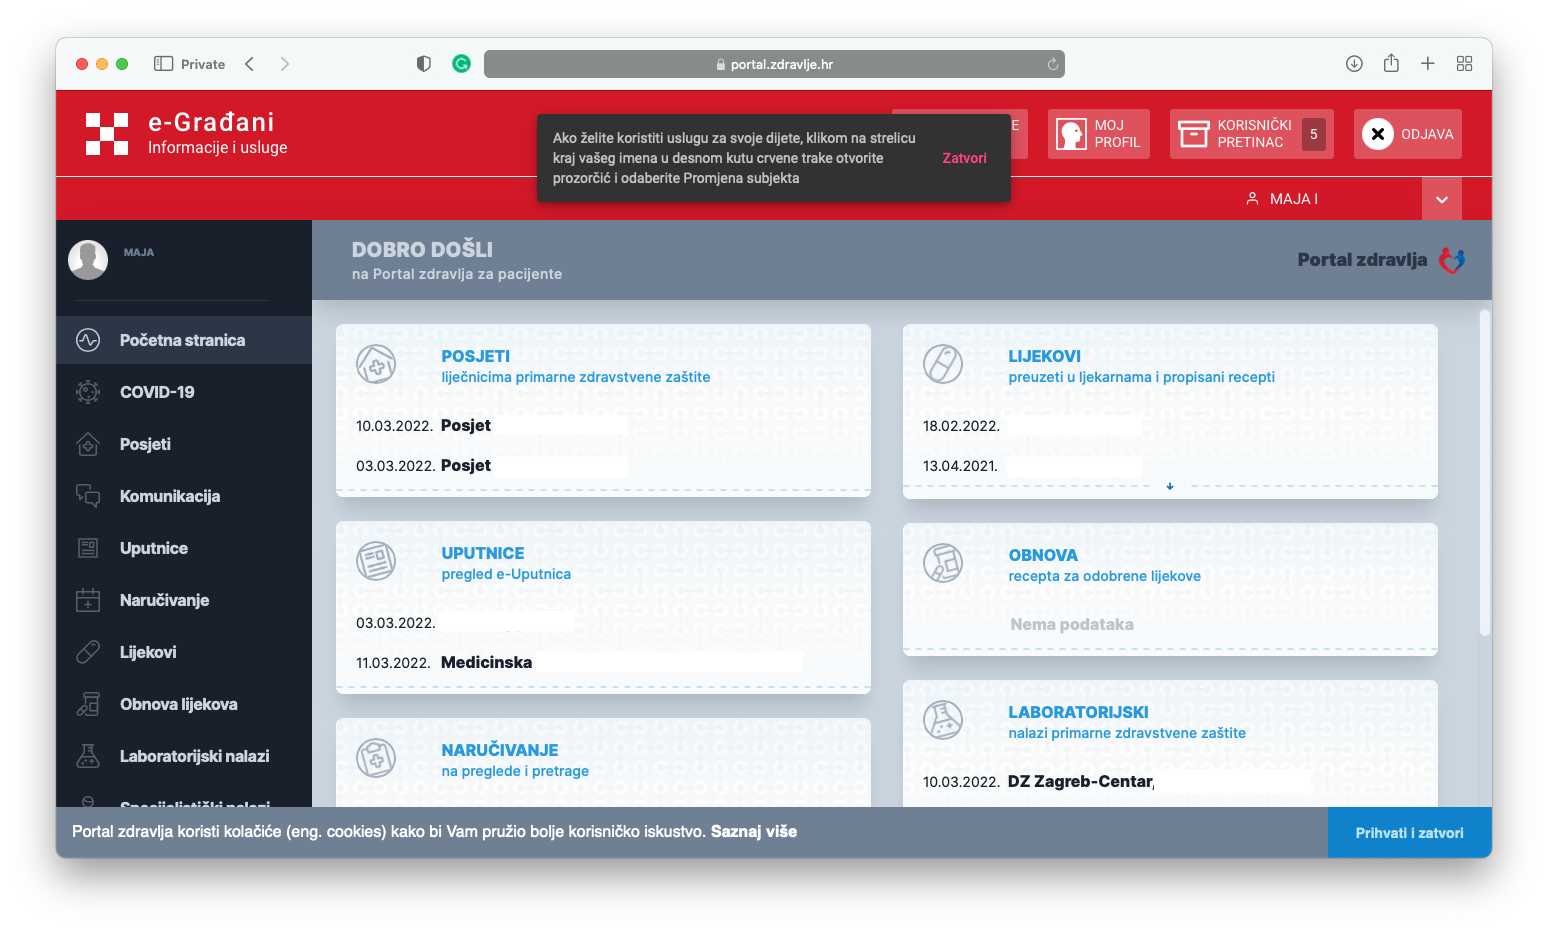
\includegraphics[width=\textwidth]{slike/portal_zdravlja.png} 
			\caption{Početna stranica "Portal zdravlje"}
\end{figure}
U konačnici, i "Ozdravi" i Portal zdravlja na e-Građani predstavljaju korisna digitalna rješenja za bolje upravljanje zdravstvenim informacijama, ali se razlikuju u svojoj svrsi, opsegu i ciljanoj publici. Oba projekta doprinose unaprjeđenju zdravstvene skrbi, svaki u svojem specifičnom kontekstu. \\
    
   Projekt "Ozdravi" je izveden kao web aplikacija, prilagođena različitim uređajima, uključujući mobilne uređaje, tablete i računalima. Osim toga, aplikacija je skalabilna i prilagodljiva za različite regije i zdravstvene ustanove.\\
    
    Opseg projektnog zadatka "Ozdravi" obuhvaća sve navedene funkcionalnosti i složenu koordinaciju između korisnika. Aplikacija omogućava brzu i preciznu komunikaciju između svih relevantnih strana. Kroz jednostavno i intuitivno sučelje, aplikacija omogućuje roditeljima, pedijatrima i liječnicima učinkovitije upravljanje zdravstvenim potrebama djece. \\
    
    Aplikacija pruža mogućnost za daljnji razvoj i proširenje, što će dodatno poboljšati iskustvo korisnika i olakšati njihovu svakodnevicu. Ova inovacija ima potencijal da unaprijedi kvalitetu života roditelja i omogući bolju skrb za djecu. Budući razvoj projekta "Ozdravi" može uključivati niz nadogradnji, uključujući integraciju s telemedicinom za daljinske konzultacije, razvoj mobilne aplikacija za veću dostupnost, proširenje podrške za različite jezike i regionalne prakse te poboljšanje analitičkih alata za praćenje medicinskih podataka. \\

	\eject
		
		
	